如图,一条直线上放着一个长和宽分别是$4$厘米和$3$厘米的长方形\ding{172},它的对角线的长恰好是$5$厘米,把这个长方形绕顶点$B$顺时针旋转$90°$后到达长方形\ding{173}的位置,这样连续做了$3$次,点$A$到达点$E$的位置,求点$A$走过的路程的长.
\begin{center}
    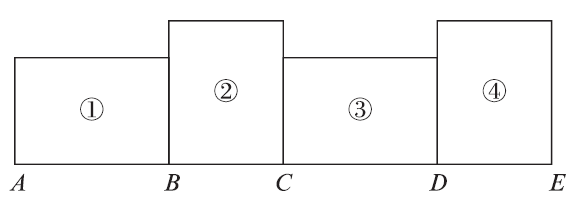
\includegraphics[height=5cm]{lib/image/MJA04010118.png}
\end{center}